\documentclass[
    language=english,
    doctype=family-tree,
    institution=none,
]{../../omnilatex}

\RequirePackage{config/document-settings}

\usepackage{tikz}
\usetikzlibrary{trees,positioning,shapes.geometric,fit,backgrounds}

\begin{document}

\maketitle

\section{The Morrison Family: A Genealogy}

\subsection{Origins}

The Morrison family traces its roots to the Scottish Highlands, where the name first appeared in historical records in the 13th century. The clan Morrison (Scottish Gaelic: \emph{Mac Ghille Mhoire}) claimed descent from the Pictish royal line and settled in the northern regions of Scotland near Durness, Sutherland.

The earliest documented ancestor in this family line is \textbf{Angus Morrison} (1780--1852), a sheep farmer who emigrated from the Isle of Skye to Nova Scotia in 1815 during the Highland Clearances. He married \textbf{Flora MacLeod} (1785--1860), and together they established a homestead in Pictou County.

\subsection{Family Tree Diagram}

\begin{center}
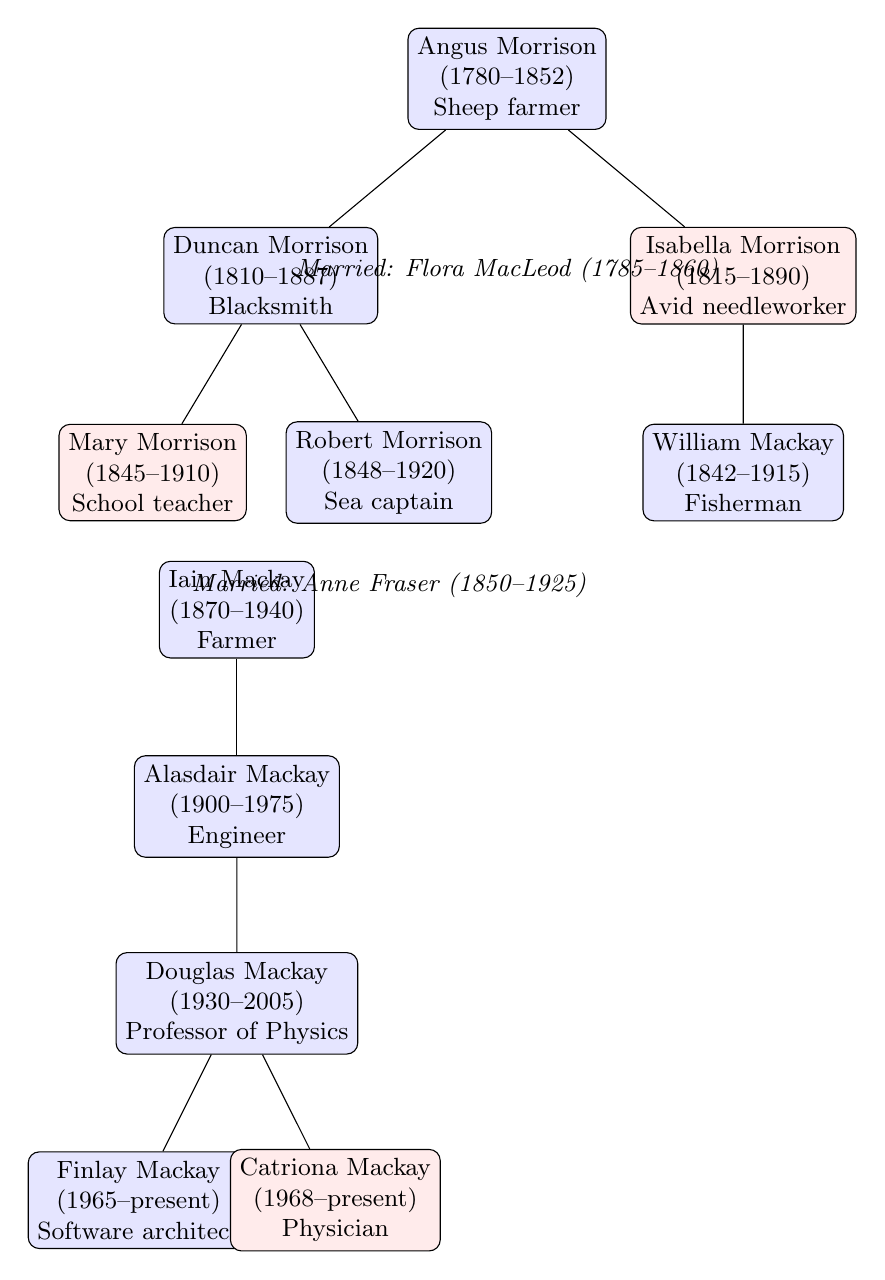
\begin{tikzpicture}[
    level 1/.style={sibling distance=6cm, level distance=2.5cm},
    level 2/.style={sibling distance=3cm, level distance=2.5cm},
    level 3/.style={sibling distance=2.5cm, level distance=2.5cm},
    every node/.style={draw, rounded corners, align=center, fill=blue!5, font=\small},
    male/.style={fill=blue!10},
    female/.style={fill=red!8},
    edge from parent/.style={draw, -}
]

\node[male] (angus) {Angus Morrison\\(1780--1852)\\Sheep farmer}
    child[male] {
        node[male] (duncan) {Duncan Morrison\\(1810--1887)\\Blacksmith}
        child[female] {
            node[female] (mary) {Mary Morrison\\(1845--1910)\\School teacher}
        }
        child[male] {
            node[male] (robert) {Robert Morrison\\(1848--1920)\\Sea captain}
        }
    }
    child[female] {
        node[female] (isabella) {Isabella Morrison\\(1815--1890)\\Avid needleworker}
        child[male] {
            node[male] (william) {William Mackay\\(1842--1915)\\Fisherman}
        }
    };

\node[below=1.5cm of angus, draw=none, fill=none, font=\small\itshape] {Married: Flora MacLeod (1785--1860)};

\node[male, below left=3cm and 4cm of isabella] (iain) {Iain Mackay\\(1870--1940)\\Farmer}
    child[male] {
        node[male] (alasdair) {Alasdair Mackay\\(1900--1975)\\Engineer}
        child[male] {
            node[male] (douglas) {Douglas Mackay\\(1930--2005)\\Professor of Physics}
            child[male] {
                node[male] (finlay) {Finlay Mackay\\(1965--present)\\Software architect}
            }
            child[female] {
                node[female] (catriona) {Catriona Mackay\\(1968--present)\\Physician}
            }
        }
    };

\node[below=0.5cm of robert, draw=none, fill=none, font=\small\itshape] {Married: Anne Fraser (1850--1925)};

\end{tikzpicture}
\end{center}

\subsection{Lineage Descriptions}

\subsubsection{The Skye Branch}

Duncan Morrison inherited his father's strength and work ethic but chose a different trade. Apprenticed to a blacksmith in Portree at age 14, he became known throughout Skye for crafting horseshoes and farm tools of exceptional quality. His workshop on Bosville Street operated continuously for 42 years.

His son Robert ran away to sea at 16 and eventually captained merchant vessels between Glasgow and the Caribbean. Robert's logbooks, preserved by the Mitchell Library, contain detailed observations of maritime trade routes in the late Victorian era.

\subsubsection{The Pictou Branch}

Isabella Morrison married William Mackay, a Gaelic-speaking fisherman whose family had fished the Northumberland Strait for generations. Their son Iain became a dairy farmer and community leader, serving as Pictou County councilor from 1905 to 1912. Iain was known for his bilingual fluency in Gaelic and English and organized the first Gaelic literary society in Nova Scotia.

\subsubsection{The Modern Generation}

Douglas Mackay, grandson of Iain, pursued academia and earned his PhD in physics from McGill University in 1956. He joined the faculty at Dalhousie University and published 47 papers on condensed matter physics. His son Finlay followed a different path into technology, co-founding a software company in Halifax that specializes in maritime navigation systems.

Catriona Mackay, Douglas's daughter, completed her medical degree at the University of Toronto and now practices family medicine in Ottawa, continuing the family tradition of community service.

\section{Family Records}

\begin{center}
\begin{tabular}{|l|l|l|l|}
\hline
\textbf{Name} & \textbf{Born} & \textbf{Died} & \textbf{Occupation} \\
\hline
Angus Morrison & 1780 & 1852 & Sheep farmer \\
Flora MacLeod & 1785 & 1860 & Homemaker \\
Duncan Morrison & 1810 & 1887 & Blacksmith \\
Isabella Morrison & 1815 & 1890 & Needleworker \\
Robert Morrison & 1848 & 1920 & Sea captain \\
Iain Mackay & 1870 & 1940 & Dairy farmer \\
Alasdair Mackay & 1900 & 1975 & Engineer \\
Douglas Mackay & 1930 & 2005 & Physics professor \\
Finlay Mackay & 1965 & --- & Software architect \\
Catriona Mackay & 1968 & --- & Physician \\
\hline
\end{tabular}
\end{center}

\section{Historical Notes}

\begin{itemize}
    \item \textbf{1815:} Angus Morrison emigrates from Skye to Nova Scotia during the Highland Clearances. The family lands were seized by the Duke of Sutherland to make way for more profitable sheep farming.
    \item \textbf{1847:} During the Great Famine, the Morrison household in Pictou sheltered three families of Irish immigrants, an act recorded in county archives.
    \item \textbf{1882:} Robert Morrison's ship \emph{The Sea Sprite} was caught in a hurricane off Bermuda. He and his crew of 14 survived by jury-rigging a replacement mast from timber on board.
    \item \textbf{1918:} Iain Mackay's eldest son enlisted in the Canadian Expeditionary Force during World War I. He survived the war and returned to farming.
    \item \textbf{1956:} Douglas Mackay defends his doctoral thesis at McGill. His research on superconductivity contributed to the development of MRI technology.
    \item \textbf{2003:} The Morrison family reunion in Pictou County drew over 200 descendants from across Canada, the United States, and Scotland.
\end{itemize}

\section{Family Motto}

\textbf{``Morior invictus''} -- I die undefeated.

This motto, adopted by the Morrison clan, reflects the resilience that has characterized the family through emigration, hardship, and the generations of rebuilding in a new land.

\end{document}
